% -*- mode: LaTeX; coding: utf-8; -*-

\chapter{Tutkimusasetelma}

Edellisissä luvuissa on esitetty pieni osa niistä hyökkäyksistä, joita vastaan verkot ja web-palvelut joutuvat nykyisin suojautumaan. Niiden suuresta määrästä johtuen on ilmiselvää, että täysin 
turvallista ympäristöä on mahdoton rakentaa. Yleensä tämä ei ole edes tietoturvasuunnittelun lähtökohtana, vaan tärkeämpää on löytää tasapaino palvelun saatavuuden, ja käytettyjen tietoturvaratkaisuiden 
välillä. Liian raskaat menetelmät aiheuttavat ylimääräistä viivettä palvelun tai verkon saatavuuteen, ja liian kevyet ratkaisut jättävät ne avoimiksi yleisimmille hyökkäyksille. 

\section{Lähtökohta}

Tämän Pro gradu-tutkielman tavoitteena on pyrkiä tunnistamaan web-palveluihin kohdistuvia poikkeavuuksia analysoimalla palvelimien tallentamaa tapahtumalokia. Analysoitava data on Apache-palvelimien 
tuottamaa lokia, joka sisältää web-palveluille kohdistuvia HTTP-pyyntöjä. Loki noudattaa CLF-formaattia (Common Log Format), jota web-palvelimet käyttävät lokitiedon tallentamiseen. Se on standardoitu 
formaatti, jossa jokaisella rivillä on tietynlainen syntaksi. Kuvassa \ref{CLF} on esitetty yhdestä HTTP-pyynnöstä syntyvä lokirivi. 

Analysoitava loki on saatu Ixonos Oy:ltä, joka tarjoaa muiden palveluiden ohella hosting-palveluita suuryrityksille. Kyseinen loki on peräisin tuotannosta jo poistetuilta palvelimilta, jotka ovat olleet
vastuussa muutaman suuren palvelukokonaisuuden pyörittämisestä. Lokia on yhteensä ?? gigatavua, ja se sisältää yli ?? miljardia sivupyyntöä, joista ??? on tullut uniikista IP-osoitteesta. Loki on kerätty
noin 10 kuukauden ajanjaksolta.

\vspace{3mm}

\begin{figure}[ht]
\centering
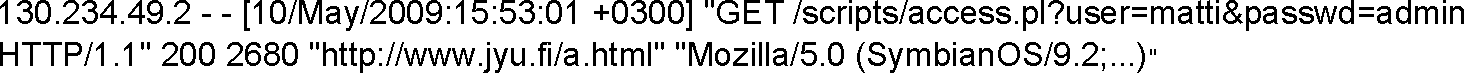
\includegraphics[width=15cm]{pics/logi.pdf}
\caption{Esimerkki web-palvelimen tuottamasta logista}
\label{CLF}
\end{figure}

Web-palvelimien tuottama loki sisältää paljon tietoa mm. palveluiden käyttöasteista, ja niihin kohdistuvista kuormista. Niitä analysoimalla voidaan myös tunnistaa mahdollisia hyökkäysyrityksiä, sekä
hyökkäyksen jo tapahduttua tutkia siihen johtaneita vaiheita. Pienillä sivustoilla lokin läpikäyminen jälkikäteen käsin on vielä mahdollista, mutta puhuttaessa palveluista, joilla on miljoonia käyttäjiä 
kuukaudessa, ei tämä ole enää mahdollista. Tästä syystä lokien analysoiminen tulee automatisoida. Tämä taas johtaa siihen, että järjestelmän tulisi pystyä tunnistamaan miljoonien kyselyiden joukosta
ne, jotka ovat syntyneet hyökkäyksen johdosta. Yksi mahdollisuus on käyttää sääntöpohjaista ratkaisua, mutta aikaisemmin esitetyistä syistä johtuen, ei tämä tarjoa aina riittävää tunnistuskykyä. Tästä 
syystä olemme päätyneet käyttämään anomalioiden tunnistamismenetelmää, jossa järjestelmälle opetetaan normaali käyttäytyminen. Tämän jälkeen haluttu data verrataan opetettuun malliin, jolloin poikkeava
liikenne voidaan tunnistaa.

Tietoturvan kannalta kiinnostavin osa logista on GET-parametrin jälkeinen osa, jossa kuljetetaan varsinainen HTTP-pyyntö. Tämä sisältää niin staattiset sivunlatauspyynnöt kuin myös palvelimelle 
välitettävät parametriarvot. Tällaisia voivat olla esimerkiksi kirjautumisessa käytetyt tiedot, ja tietokannalle välitetyt kyselyt. Staattiset sivunlatauspyynnöt ja parametreja sisältävät pyynnöt erottaa
resurssipolun jälkeisestä kysymysmerkistä. Kysymysmerkin jälkeinen kyselyosuus koostuu avain-arvo-pareista, joista ensimmäinen on kutsuttu parametri, ja jälkimmäinen tämän arvo (kuva \ref{CLF2}). Riippuen
palvelun toteutuksesta näitä voi olla useampia peräkkäin \&-merkillä erotettuna.

\begin{figure}[ht]
\centering
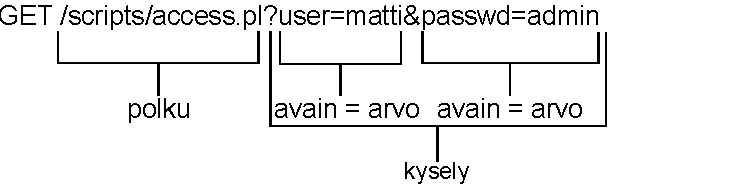
\includegraphics[width=13cm]{pics/logi2.pdf}
\caption{HTTP-kyselyn GET-osa}
\label{CLF2}
\end{figure}

\section{Käytettyjen menetelmien yleinen kuvaus}

Anomalioiden tunnistamiseen käyttämämme järjestelmä pohjautuu diffuusiokuvausten käyttöön, joiden avulla on mahdollista tunnistaa poikkeavuudet normaalin liikenteen joukosta. 

\subsection{Diffuusiokuvaus}

\subsection{n-gram analyysi}

\subsection{Satunnaisprojektio}



%- mistä lähtökohdista lähdetään tutkimaan eli mitä materiaalia on käytössä
%- mitä voidaan etsiä käytössä olevasta materiaalista
%- mitä menetelmiä käytetään (n-gram, diffuusiokuvaus, satunnaisprojektio)
%- korkeamman tason selitys mitä tehdään
%- menetelmien tarkka kuvaus
